\documentclass[output=paper,colorlinks,citecolor=brown]{langscibook}
\ChapterDOI{10.5281/zenodo.15006615}

\author{Akiko Takemura\orcid{}\affiliation{Université d'Orléans; Kobe University}}
\title[Information about grandparents when selecting a dialect speaker]
      {How important is information about grandparents when selecting a dialect speaker?}

\abstract{This paper aims at setting a new criterion for selecting a local dialect speaker by inquiring about the origin of their parents, which accommodates to the reality in large cities. In Japanese dialectology, it is widely accepted that a dialect speaker should ideally be \emph{haenuki} (`native-born'), i.e. a person from a family who has lived in the survey area for three generations. However, this criterion has been used hitherto without checking the assumptions that it is both justified and useful. After reexamining the data collected from three families by the \citet{NLRI1965} and conducting one survey, I conclude that the \emph{haenuki} criterion is impractical, and not fully justified and that the most important criterion when selecting a representative speaker of a dialect should be having both parents native born.}


\IfFileExists{../localcommands.tex}{
   \addbibresource{../localbibliography.bib}
   \usepackage{tabularx,multicol}
%\usepackage{multirow}
\usepackage{subcaption}
\usepackage{url}
\urlstyle{same}

\usepackage{datetime}
\usepackage{enumitem}
\usepackage{langsci-optional}
\usepackage{langsci-lgr}
\usepackage{langsci-branding}

\usepackage{longtable}
\usepackage{xltabular}
\usepackage[linguistics, edges]{forest}
\usepackage{pgfplots}
\pgfplotsset{compat=1.18}
\usetikzlibrary{patterns, tikzmark}
\usepackage{pgfplotstable}
\usepgfplotslibrary{colorbrewer}
\usepackage{listings}
\lstset{basicstyle=\ttfamily,keywordstyle=\normalfont,language=,breaklines=true}

\usepackage{siunitx}
\sisetup{group-digits=none, detect-all=true}

\usepackage{langsci-gb4e}

   \makeatletter
\let\thetitle\@title
\let\theauthor\@author
\makeatother

% Use this Chinese font shipped with TeX Live instead of Source Han, because
% it is more portable/leightweight. Install the "fandol" package from CTAN to
% automatically get this font.
\newfontfamily{\ChineseFandolSong}{FandolSong-Regular.otf}

   %% hyphenation points for line breaks
%% Normally, automatic hyphenation in LaTeX is very good
%% If a word is mis-hyphenated, add it to this file
%%
%% add information to TeX file before \begin{document} with:
%% %% hyphenation points for line breaks
%% Normally, automatic hyphenation in LaTeX is very good
%% If a word is mis-hyphenated, add it to this file
%%
%% add information to TeX file before \begin{document} with:
%% %% hyphenation points for line breaks
%% Normally, automatic hyphenation in LaTeX is very good
%% If a word is mis-hyphenated, add it to this file
%%
%% add information to TeX file before \begin{document} with:
%% \include{localhyphenation}
\hyphenation{
    a-na-ly-sis
    ap-proach-es
    ar-che-o-log-i-cal
    Ar-khan-gelsk
    be-schrei-ben
    Buch-holtz
    Che-lya-binsk
    con-so-nant
    dia-lect
    dia-lect-ology
    Di-a-lekt-for-schung
    Dia-lekt-for-schung
    East-pha-lian
    För-der-ung
    Ge-mein-schaft-lich-keits-ent-wür-fe
    his-tor-i-cal
    Hok-kai-do
    ja-pa-nese
    Ja-pa-nese
    Ka-go-shi-ma
    Ka-li-nin-grad
    Knja-zev
    Ma-kro-be-reich
    Ma-lay-sia
    mor-pho-log-i-cal
    Mos-cow
    Nef-te-yu-gansk
    non-mobile
    nu-cle-ar
    ös-ter-rei-chi-sche
    par-a-digm
    per-zep-ti-ons-lin-gu-is-ti-sche
    plu-ri-zen-tri-schen
    quick-ly
    Reich
    Sax-on
    Schrö-der
    sear-ching
    ste-reo-type
    strength-en-ing
    strong-est
    Stutt-gart
    su-pra-seg-men-tal
    teach-er
    to-po-gra-phy
    To-ron-to
    tra-di-tion-al
    ul-ti-mate-ly
    Um-gangs-spra-che
    Volks-kun-de
    vor-zu-stel-len
    wheth-er
    Wie-sing-er
    with-in
    Wort-at-las
}

\hyphenation{
    a-na-ly-sis
    ap-proach-es
    ar-che-o-log-i-cal
    Ar-khan-gelsk
    be-schrei-ben
    Buch-holtz
    Che-lya-binsk
    con-so-nant
    dia-lect
    dia-lect-ology
    Di-a-lekt-for-schung
    Dia-lekt-for-schung
    East-pha-lian
    För-der-ung
    Ge-mein-schaft-lich-keits-ent-wür-fe
    his-tor-i-cal
    Hok-kai-do
    ja-pa-nese
    Ja-pa-nese
    Ka-go-shi-ma
    Ka-li-nin-grad
    Knja-zev
    Ma-kro-be-reich
    Ma-lay-sia
    mor-pho-log-i-cal
    Mos-cow
    Nef-te-yu-gansk
    non-mobile
    nu-cle-ar
    ös-ter-rei-chi-sche
    par-a-digm
    per-zep-ti-ons-lin-gu-is-ti-sche
    plu-ri-zen-tri-schen
    quick-ly
    Reich
    Sax-on
    Schrö-der
    sear-ching
    ste-reo-type
    strength-en-ing
    strong-est
    Stutt-gart
    su-pra-seg-men-tal
    teach-er
    to-po-gra-phy
    To-ron-to
    tra-di-tion-al
    ul-ti-mate-ly
    Um-gangs-spra-che
    Volks-kun-de
    vor-zu-stel-len
    wheth-er
    Wie-sing-er
    with-in
    Wort-at-las
}

\hyphenation{
    a-na-ly-sis
    ap-proach-es
    ar-che-o-log-i-cal
    Ar-khan-gelsk
    be-schrei-ben
    Buch-holtz
    Che-lya-binsk
    con-so-nant
    dia-lect
    dia-lect-ology
    Di-a-lekt-for-schung
    Dia-lekt-for-schung
    East-pha-lian
    För-der-ung
    Ge-mein-schaft-lich-keits-ent-wür-fe
    his-tor-i-cal
    Hok-kai-do
    ja-pa-nese
    Ja-pa-nese
    Ka-go-shi-ma
    Ka-li-nin-grad
    Knja-zev
    Ma-kro-be-reich
    Ma-lay-sia
    mor-pho-log-i-cal
    Mos-cow
    Nef-te-yu-gansk
    non-mobile
    nu-cle-ar
    ös-ter-rei-chi-sche
    par-a-digm
    per-zep-ti-ons-lin-gu-is-ti-sche
    plu-ri-zen-tri-schen
    quick-ly
    Reich
    Sax-on
    Schrö-der
    sear-ching
    ste-reo-type
    strength-en-ing
    strong-est
    Stutt-gart
    su-pra-seg-men-tal
    teach-er
    to-po-gra-phy
    To-ron-to
    tra-di-tion-al
    ul-ti-mate-ly
    Um-gangs-spra-che
    Volks-kun-de
    vor-zu-stel-len
    wheth-er
    Wie-sing-er
    with-in
    Wort-at-las
}

   \boolfalse{bookcompile}
   \togglepaper[23]%%chapternumber
}{}

\begin{document}
\maketitle
\label{chap:takemura}
\graphicspath{{figures/takemura}}

\section{Introduction}

Dialect surveys crucially rely on a sample of speakers taken to be representative of a dialect. The criteria used for selecting a representative speaker and the very definition of who can be considered to be a speaker of a dialect are important methodological issues. In Japanese dialectology, it is widely accepted that a dialect speaker should ideally be \emph{haenuki} (`native born'), i.e., a person from a family who has lived in the survey area for three generations. However, this criterion has been used hitherto without checking whether it is both justified and useful. In this paper, I would like to discuss whether it is useful to take into account information about a speaker's grandparents in dialect surveys.

After reviewing in detail the existing literature on the \emph{haenuki} criterion and its motivation, I present the results of a reexamination of data obtained by the \citet{NLRI1965}  and of a survey, conducted by the author, of Japanese dialects intended to clarify whether it is indeed justified: the former is on the transmission of lexical accent across three generations, and the latter is on the transmission of lexical accent and phonological rules across two generations. In view of these results, I conclude that the \emph{haenuki} criterion is unpractical and not fully justified, especially in large cities, and that the most important criterion for selecting a representative speaker of a dialect should be having both parents native born.

\section{Criteria for a representative speaker of a dialect}

\tabref{tab:haenuki} details the different criteria proposed in the Japanese literature to determine whether a speaker can be taken or not as a representative of a dialect.\footnote{\textcite{Yoshida1984} says that the influence of parents and spouses is very limited, but also that the origins of parents and spouses should be taken into account when researching accents. It is somewhat contradictory, but I assume that the former concerns the influence on the acquisition of grammar or lexical items.} In Japanese dialectology, a speaker is considered representative of a dialect if they, along with their parents and grandparents, were born and raised in the survey area. However, this widely accepted criterion has been adopted without much justification and its usefulness remains to be shown.

\begin{table}
\centering
\caption{Criteria for dialect speakers}
\label{tab:haenuki}
\begin{tabularx}{\textwidth}{ lQ }
\lsptoprule
Source & Criterion \\ \midrule
\multicolumn{2}{l}{\citet{NLRI1981}}\\
  & lexical accent is influenced by where a person spent their language formation period, and not by any afterward relocation \\\addlinespace
\multicolumn{2}{l}{\citet{Uwano1984}, \citet{Uwano1997}} \\
&  %Criteria: \emph{haenuki}
\begin{itemize}[nosep, noitemsep,leftmargin=0pt]
  \item speakers who have lived in the area throughout their so-called ``language formation period"
  \item it is ideal if both the parents and grandparents are from the location; parental influence is weak, especially the father’s influence, as it is seen in the vocabulary used only at home
  \item ``people who have lived somewhere else than their birth place at least once" because they are more sensitive to variation
(assuming that those people often have a better sense of language)
\end{itemize} \\\addlinespace
\multicolumn{2}{l}{\citet{Yoshida1984}} \\
 &  \begin{itemize}[nosep, noitemsep,leftmargin=0pt]
  \item ideally, \emph{haenuki}
  \item people who have lived in the area until the age of language formation (around 13 years old) and have little history of living outside
  \item influence of parents and spouse is very limited
  \item note that the influence of parents’ language is more important in surveys of young people
  \item origins of parents and spouses should be taken into account when it comes to accentual research
\end{itemize} \\
\lspbottomrule
\end{tabularx}
\end{table}

The strict application of this criterion poses the practical problem that in some cases such speakers are rare or even nonexistent (\citealt{Sibata1984}, \citealt{Sibata1988}), especially nowadays due to the increased mobility of populations for reasons of marriage, education, work, etc. For example, \citet[64, my translation]{Sibata1984} reports that ``in 1965, no one met the criteria of being over 65 years old and \emph{haenuki} in the surroundings of the Urawa Station in Saitama prefecture'', and similarly \citet[566, my translation]{Sibata1988} reports that:

\begin{quote}
We have been able to find many natives who were born in the area and have lived there for a long time, but from now on there will be fewer people who meet these conditions. [\ldots] Even if the conditions are relaxed, I do not think it will be possible to find anyone who meets the conditions in the future.
\end{quote}

Outside the circles of Japanese dialectology, the NORM (Non-mobile, Old, Rural, Men) criterion is widely used in dialect research, but it is difficult to apply in the case of large cities. To capture the linguistic dynamics in large cities, \citet[40--46]{ChambersHeisler1999} proposed the Regionality Index (RI):

\begin{quote} 
In the Dialect Topography sample, we aim for a demographic cross section of the survey area rather than a population of indigènes as in traditional dialect surveys. Our reasoning is straightforward: some proportion of urban speech communities is made up of people who were born outside the community, and the variants they use in their speech are heard in that speech community and have some status in it. We want to know what those variants are and the extent of their use. Our quantitative model allows us to distinguish indigènes and interloper variation by correlating variants with the provenance (via RI) of the respondents who use them.
\end{quote}

The RI is thus a measure of the degree of representativeness of a speaker for a given dialect based on the speaker's background factors such as birthplace, current residence during the survey, upbringing between the ages of 8 to 18, and the birthplace of their parents. The RI is computed using this information and yields values ranging from 1 to 7. The lower the RI value, the greater the speaker's nativeness. To illustrate, consider a speaker with an RI value of 1. This individual is not only born and raised in the same location as this individual's parents, but also lives there currently, reflecting a strong local connection. Conversely, an RI value of 7 denotes an individual who resides within the surveyed region but was born and raised outside the area, with parents also coming from the other area. The RI aids in distinguishing speech variants employed by natives versus newcomers, making it particularly suitable for extensive investigations within large cities. However, it may not prove optimal for smaller-scale studies where the selection of a limited number of representative speakers is unavoidable.

As noted previously, the \emph{haenuki} criterion has been used in Japan in dialect research without much consideration. Yet, its applicability in contemporary times, specifically in conducting dialect research in large cities, raises considerable challenges. The scarcity of people who satisfy such strict criteria makes its feasibility questionable. Consequently, inquiries into the credibility of this criterion are well-founded. In an effort to assess its validity, this study aims to address two key research questions:

\begin{enumerate}
    \item How important is information about grandparents? 
    \item Do parents’ origins matter in dialect acquisition? 
\end{enumerate}

To answer the first question, I reexamined the data collected in the 1960s \citep{NLRI1965} on lexical accent transmission across three generations in three different locations in Hokkaido (Section 3). I then investigated the influence of parents on the acquisition of lexical accent and phonological rules in young speakers in Kagoshima (Section 4) \citep{Takemura2012} to answer the second question.


\section{Transmission of lexical accent across three generations in Hokkaido}\label{sec:hokkaido}

The \citet{NLRI1965} presents data collected in the 1960s on three different families located in three locations on Hokkaido Island in order to study the process of language standardization. Hokkaido was traditionally inhabited by the indigenous Ainu people, and it was only during the Meiji era (1868--1912) that Japanese speakers began to settle in Hokkaido. The settlers came from all over Japan bringing with them their own dialect. Therefore, Hokkaido at that time was a linguistically heterogeneous place without any characteristic dialect, and a standard language emerged.

\begin{figure}
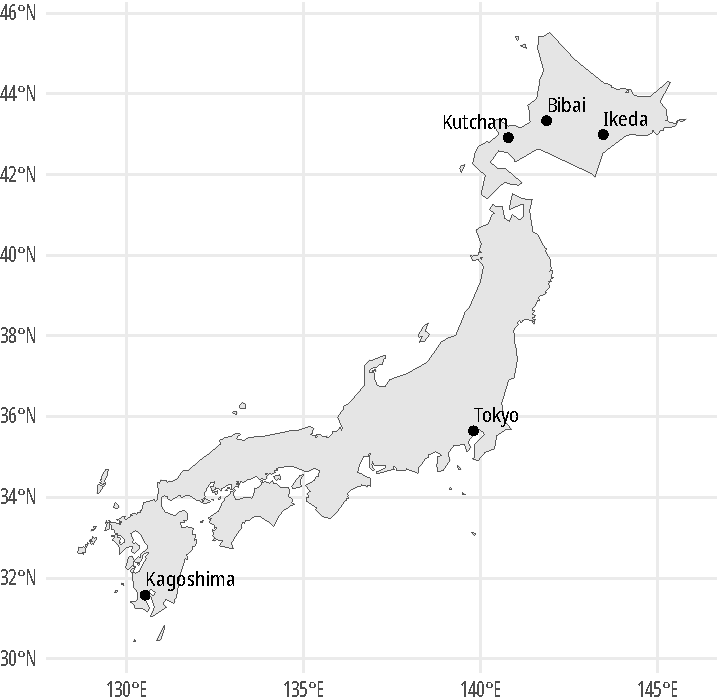
\includegraphics[width=\textwidth]{takemura-japan.pdf}
\caption{Map of Japan showing Tokyo and the locations of the surveys}
\label{fig:japan}
\end{figure}

The \citet{NLRI1965} researchers collected data from three locations in Hokkaido: Bibai, Ikeda and Kutchan (\figref{fig:japan}). At each location, a family of three generations participated in the survey. They were asked to pronounce each word on wordlists, and researchers wrote down the accent patterns observed, and I compared to what extent the accent patterns for a given word match across the different generations.

There are gaps in the data for the \citet{NLRI1965}, so I focused on those lexical items for which we have information on their accentuation in at least two generations and compared the agreement ratio as follows. Agreement ratio is calculated: the denominator corresponds to the total number of lexical accents obtained between the given two generations. Meanwhile, the numerator hinges on the tally of lexical items articulated in the same manner across the two generations. To illustrate, consider the lexical item \emph{hinomaru} (`the rising-sun flag'). For the first generation of the family from the town of Ikeda, the pronunciation follows the pattern Low-High-High-Low (abbreviated as LHHL hereafter). However, the second and third generations pronounce it as LHHH. Consequently, there is no concurrence between the first generation and the subsequent two generations.

Certain lexical items lack accent information for specific generations.
%(For more details, see \figref{fig:datahokkaido} in appendix). 
For instance, for the word \emph{tomodachi} (`friend'), the first generation's recorded accent is LHHL, while the third generation's is LHHH. However, there is no available information for the second generation. In such cases, the agreement ratio cannot be computed between the first and second generations, or between the second and third generations. Nonetheless, the calculation of the agreement ratio between the first and third generations remains possible. \figref{fig:hokkaido} summarizes the results, and more details can be found in the appendix.

\begin{figure}
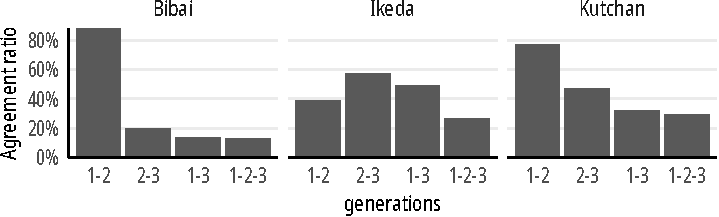
\includegraphics[width=\textwidth]{takemura-hokkaido.pdf}
\caption{Agreement ratio in accentuation between generations in Hokkaido; generation 1 is that of the grandparents, 2 that of the parents, and 3 that of the children}
\label{fig:hokkaido}
\end{figure}

The transmission of dialect accentuation from grandparents to grandchildren differs from family to family, but we can still notice some trend in the data. There is a larger ratio disagreement than agreement ratio between the first and third generations in all three families, which shows that accent transmission is imperfect between the first and third generations. Interestingly, a family from Ikeda town shows a reverse trend from other families for the agreement between the first and second generations. Whereas the agreement ratio between the first and second generations is usually higher than between the first and third generations, in the family from Ikeda it is the opposite, in accord with the findings of \citet{InoueHanzawa2022} that the speech of children raised with their grandparents is influenced by that of their grandparents.

Revisiting the initial research question posited in the previous section -- the significance of information about grandparents -- a definitive answer remains elusive. However, an overarching trend emerges indicating that accentuation transmission encounters imperfections between the first and third generations. This implies that intergenerational influence is more restricted to adjacent generations.

\section{Parental influence in the acquisition of lexical accent and phonological rule in Kagoshima}\label{sec:kagoshima}

If, as seen in the previous section, there is an influence between adjacent generations, we expect that parental origins play an important role in dialect acquisition. On the other hand, if a child acquires its local dialect from his peers, there should be no difference between the children with locally born parents and those with non-locally born parents as to their dialect acquisition. I can thus categorize children into four groups depending on their parental origins (\tabref{tab:categ}). Group 1 in \tabref{tab:categ} has both locally born parents. Group 2 has a local mother but non-local father. Group 3 has a non-local mother but a local father. Lastly, Group 4 has neither a local mother nor a local father. 

\begin{table}
\centering
\caption{Child categorization according to their parental origins}
\label{tab:categ}
\begin{tabular}{llll}
\lsptoprule
& & \multicolumn{2}{c}{Father} \\\cmidrule(lr){3-4}
& & Local & Non-local \\ \midrule
Mother & Local & Group 1 & Group 2 \\
       & Non-local & Group 3 & Group 4 \\
\lspbottomrule
\end{tabular}
\end{table}

Here I present the results of the survey by \citet{Takemura2012} on accent acquisition of the Kagoshima dialect in Japan (\figref{fig:japan}). It focuses on two aspects: acquisition of the lexical accents of words, which is stored in the mental lexicon as a part of lexical representations, and acquisition of productive accent rules, which must be inferred from the linguistic input. The survey aims at answering the following questions:
\begin{enumerate}
  \item Do parental origins influence accent acquisition?
  \item If parental origins matter in dialect accent acquisition, is there a difference between the acquisition of lexical accent and the acquisition of phonological rules?
\end{enumerate}

Whereas Tokyo Japanese is mora-based and has a free pitch accent system, the Kagoshima dialect is syllable-based and has only two possible pitch patterns: Pattern A with a high pitch on the penultimate syllable and Pattern B with a high pitch on the final syllable. Contrary to Tokyo Japanese, the location of the high pitch shifts when a particle is added to a word since the domain of pattern is the prosodic word (Tables \ref{tab:tabemono} and \ref{tab:nomimono}).\footnote{\citet{Takemura2012} also presents data on the acquisition of rule-based accentuation of compounds. However, the acquisition of compound accentuation is also affected by the confounding factor of ongoing influence of Tokyo Japanese \citep{Kubozono2006}, which makes those data more problematic than useful to be included in the present study.}

For example, \emph{tabemóno} (`food'), in Table \ref{tab:tabemono}, is traditionally a Pattern A word. Within this word, the penultimate syllable \emph{mó} is pronounced with high pitch, as indicated by the acute accent on the vowel. When we add a nominative particle \emph{ga} after \emph{tabemóno}, then the high pitch shifts to \emph{nó} because it is now the penultimate syllable. Pattern B behaves similarly, with the high pitch shifting to the final syllable depending on word length, e.g. \emph{nomimonó} (`beverage') but \emph{nomimono=gá} in Table \ref{tab:nomimono}.

\begin{table}
\centering
\caption{Kagoshima Pattern A: High pitch on the penultimate syllable}
\label{tab:tabemono}
\begin{tabular}{lll}
\lsptoprule
                & Form            & Gloss      \\\midrule
in isolation    & \textit{tabemóno}    & `food'     \\
with a particle & \textit{tabemonó=ga} & `food=\textsc{nom}' \\
\lspbottomrule
\end{tabular}
\end{table}

\begin{table}
\centering
\caption{Kagoshima Pattern B: High pitch on the final syllable}
\label{tab:nomimono}
\begin{tabular}{lll}
\lsptoprule
                & Form            & Gloss      \\\midrule
in isolation    & \textit{nomimonó}    & `beverage'     \\
with a particle & \textit{nomimono=gá} & `beverage=\textsc{nom}' \\
\lspbottomrule
\end{tabular}
\end{table}

Tables \ref{tab:tabenomi} and \ref{tab:nominomi} illustrate how I checked the acquistion of phonological rule. When a speaker pronounces `food' as \emph{tabemóno} in isolation and as \emph{tabemonó=ga} with a particle, I thus conclude that the speaker has acquired the phonological rule since the location of the high pitch shifts according to the length of the prosodic word. However, if the pronunciation is \emph{tabemóno=ga} with no shift, then I conclude that even though the speaker has acquired the traditional lexical accent, the speaker has not acquired the phonological rule. In the case of a speaker pronouncing \emph{tabemonó} and \emph{tabemono=gá}, it signifies the attainment of the phonological rule but not the acquisition of lexical accent. Conversely, if the pronunciation is \emph{tabemonó} and \emph{tabemonó=ga}, it implies the speaker has not acquired either the lexical accent or the phonological rule. I use the same criteria for Pattern B words such as \emph{nomimonó} (`beverage') (Table \ref{tab:nominomi}).



\begin{table}[p]
\centering
\caption{Criteria for process of the acquisition of Pattern A}
\label{tab:tabenomi}
\begin{tabular}{llll}
\lsptoprule
In isolation & With a particle & Lexical accent & Phonological rule \\\midrule
\emph{tabemóno} & \emph{tabemonó=ga} & YES & YES \\
\emph{tabemóno} & \emph{tabemóno=ga} & YES & NO \\
\emph{tabemonó} & \emph{tabemono=gá} & NO & YES \\
\emph{tabemonó} & \emph{tabemonó=ga} & NO & NO \\
\lspbottomrule
\end{tabular}
\end{table}

\begin{table}[p]
\centering
\caption{Criteria for process of the acquisition of Pattern B}
\label{tab:nominomi}
\begin{tabular}{llll}
\lsptoprule
In isolation & With a particle & Lexical accent & Phonological rule \\\midrule
\emph{nomimonó} & \emph{nomimono=gá} & YES & YES \\
\emph{nomimonó} & \emph{nomimonó=ga} & YES & NO \\
\emph{nomimóno} & \emph{nomimonó=ga} & NO & YES \\
\emph{nomimóno} & \emph{nomimono=gá} & NO & NO \\
\lspbottomrule
\end{tabular}
\end{table}

\begin{table}[p]
\caption{Participants in the Kagoshima survey}
\label{tab:kagpart}
\begin{tabular}{lllll}
\lsptoprule
                        &                            & \multicolumn{2}{c}{Father} & Total      \\\cmidrule(lr){3-4}
                        &                            & Local        & Nonlocal   &            \\\midrule
                 Mother & Local                      & Group 1: 18  & Group 2: 13 & 31         \\
                        &                            & Male: 4      & Male: 2     & Male: 6    \\
                        &                            & Female: 14   & Female: 11  & Female: 25 \\\cmidrule(lr){2-5}
                        &                   Nonlocal & Group 3: 16  & Group 4: 8  & 24         \\
                        &                            & Male: 4      & Male: 3     & Male: 7    \\
                        &                            & Female: 12   & Female: 5   & Female: 17 \\\midrule
                 Total  &                            & 34           & 21          & 55         \\
                        &                            & Male: 8      & Male: 5     & Male: 13   \\
                        &                            & Female: 26   & Female: 16  & Female: 42 \\
\lspbottomrule
\end{tabular}
\end{table}

There were 55 participants aged between 15 and 28 years old, whose family background is summarized in Table \ref{tab:kagpart}. \figref{fig:kagoshima} summarizes the results of isolated forms, which reflect the acquisition of lexical accent. It indicates the agreement ratio of productions that matches the traditional pattern. We observe that Group 1 (both parents locally born) is the most conservative and that Group 4 (no parent locally born) is the most innovative. A Tukey test shows that Group 1 differs significantly from Groups 3 and 4 ($p < 0.001$).\footnote{A Tukey HSD test was used to correct for multiple comparisons. There was also a statistically significant difference between Group 2 and Group 4 ($p < 0.05$), but no statistically significant differences were observed between any other two groups..} Thus, even though all informants grew up in the Kagoshima area, the acquisition of lexical accent differs between those with non-local parents.

Concerning the acquisition of the phonological rule of pitch shift in prosodic words with a particle, Group 4 (non-local parents) is again the most innovative and Group 1 is the most conservative (\figref{fig:kagoshima}), and the difference between the two is statistically significant (Tukey test, $p < 0.001$).

\figref{fig:kagoshima2} compares for each group the ratio of realizations matching the traditional patterns. Group 1 behaves differently compared to the other groups, since there is a better match with the traditional pattern for the phonological rule than for the lexical accent.

\begin{figure}
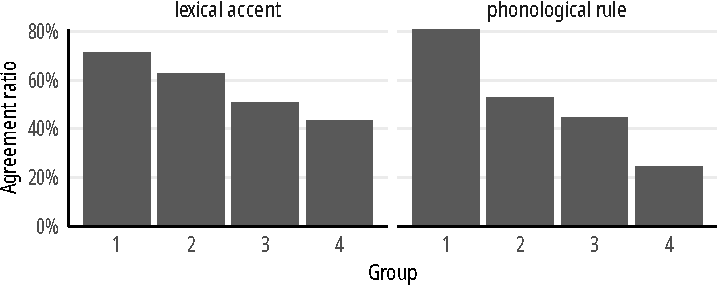
\includegraphics[width=0.8\textwidth]{takemura-kagoshima.pdf}
\caption{Acquisition of lexical accent and phonological rule}
\label{fig:kagoshima}
\end{figure}

\begin{figure}
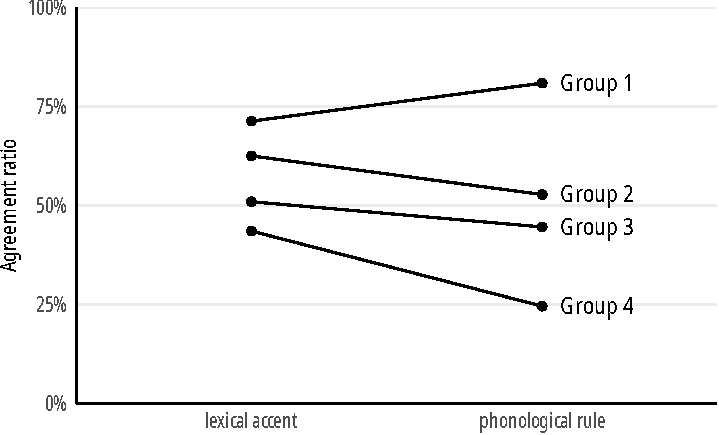
\includegraphics[width=0.8\textwidth]{takemura-kagoshima2.pdf}
\caption{Acquisition of lexical tone vs. acquisition of phonological rule in Kagoshima}
\label{fig:kagoshima2}
\end{figure}
\pagebreak
The Kagoshima survey therefore shows evidence that parental origins do influence dialect acquisition for both lexical accent and phonological rule. These results agree with the conclusions of \citet{Trudgill1986} on Norwich English and \citet{SugitoOkumura1984} on Kansai Japanese. Moreover, the acquisition of phonological rules seems to pose problems for speakers with non-local parents, in agreement with the results of \citet{Payne1976} on Philadelphia English and of \citet{Takemura2010} on Kansai Japanese. It can be hypothesized that those speakers with locally born parents were raised in an environment relatively free of influence from other dialects, which fosters a relatively faithful acquisition of the traditional dialect. On the other hand, speakers with at least one non-local parent were raised in a dialect contact environment, which challenges faithful transmission. Speakers with both native parents nevertheless also show some effects of internal changes in the accent category membership of lexical items, but transmission of phonological rules appears to be stable. Speakers with at least one non-native parent seem to have not fully acquired the traditional tone rule. This trend fits the common knowledge in historical linguistics \citep{Hock1991} that rules are more resistant to both internal diachronic change (people with locally born parents) and to borrowing (people with at least one non-local parent). 

\section{Conclusions}

The present study questioned whether the \emph{haenuki} criterion widely held in Japanese dialectology, i.e., that in order to be considered as representative of a given dialect, a speaker should have native-born parents and grand-parents, is truly justified and thus whether information about a speaker's grandparents is really important and useful for dialect research. We first saw that the \emph{haenuki} criterion poses problems in the context of dialect surveys in large cities since it is often the case that few, if any, speakers satisfy this criterion, so that it is not practically applicable in many real-life situations.

\begin{sloppypar}
The reexamination of data on lexical accent acquisition across three generations in Hokkaido shows limited transmission between the first generation (grandparents) and the third generation (children) in two families out of three, though there seems to be some influence between adjacent generations, i.e. between grandparents and parents and between parents and children. It is likely that the origin of grandparents is not important in itself, but whether a child was raised with his grandparents \citep{InoueHanzawa2022}. In this case, the information regarding the grandparents' origins would not offer substantial assistance on its own. However, in all the three families included in the Hokkaido survey, the three generations of grandparents, parents, and children lived together, and the reasons for the limited transmission of accentuation between grandparents and children remain to be investigated. We should also keep in mind that Hokkaido constitutes a peculiar case since it was settled by Japanese speakers only in the second half of the 19th century, and for a long period there was no Hokkaido dialect proper. Data from a region with a traditional dialect might bring different results. However, this does not alter the conclusion that grandparents might not always have a significant impact on dialect transmission. It suggests that incorporating details about grandparents might not always be essential or beneficial when selecting a representative speaker.
\end{sloppypar}

The results of the survey on the acquisition of lexical accent and phonological rule in young speakers of Kagoshima Japanese show the determining influence of the parents' origins. Speakers with both native parents show the most faithful acquisition of both the lexical accent and phonological rule of the traditional dialect, and those without a native parent show the least faithful acquisition. Moreover, there is a stark distinction between speakers with both native parents and all the other groups: for all the other groups, speakers show a less faithful acquisition of the phonological rule than that of the lexical accent of words, but the situation is reversed for those speakers whose both parents are native-born. This suggests that the acquisition of phonological rules, i.e., grammar, is strongly influenced by the origins of the parents, much more than lexical acquisition.

Both of the two surveys examined above highlight the role of intergenerational transmission in dialect acquisition, and indicate that we cannot consider a speaker as representative of a dialect solely based on whether they are themselves native-born. When looking at the result of the reexamination of data in Hokkaido, it becomes apparent that a speaker's grandparents' origins have a smaller impact on dialect accent acquisition, more specifically lexical accent acquisition, compared to their parents' origins. Moreover, from the result of Kagoshima survey I observed differences in dialect acquisition between speakers with both native-born parents and all others, even those with one native-born parent and a non-native one, especially in the acquisition of phonological rules. 
We can conclude that the \emph{haenuki} criterion is not only unpractical but also not fully justified, and that the most important criterion when selecting a representative speaker of a dialect should be to have both parents native-born.

\section*{Appendix}
\largerpage[2]

\begin{table}[H]
\caption{Data of the family in Bibai}
\begin{tabular}{l  *3{r@{~}l} }
\lsptoprule
Generations & \multicolumn{2}{c}{Agreement} & \multicolumn{2}{c}{Disagreement} & \multicolumn{2}{c}{Total} \\ \midrule
1--2 & 443 & (87.9\%) & 61 & (12.1\%) & 504 & (100.0\%)\\
2--3 & 96 & (19.9\%) & 386 & (80.1\%) & 482 & (100.0\%) \\
1--3 & 67 & (13.9\%) & 415 & (86.1\%) & 482  & (100.0\%)\\
1--2--3 & 63 & (13.1\%) & 413 & (85.7\%)  & 476 & (100.0\%) \\
      
\lspbottomrule
\end{tabular}
\end{table}

\begin{table}[H]
\caption{Data of the family in Ikeda}
\begin{tabular}{l  *3{r@{~}l} }
\lsptoprule
Generations & \multicolumn{2}{c}{Agreement} & \multicolumn{2}{c}{Disagreement} & \multicolumn{2}{c}{Total} \\ \midrule
1--2 & 56   & (38.6\%) & 89 & (61.4\%) & 145 & (100.0\%)  \\
2--3 & 113  & (57.4\%) & 84 & (42.6\%) & 197 & (100.0\%)\\
1--3 & 89   & (49.2\%) & 92 & (50.8\%) & 181 & (100.0\%) \\
1--2--3 & 34 & (26.8\%) & 93 & (73.2\%) & 127 & (100.0\%) \\
\lspbottomrule
\end{tabular}
\end{table}

\begin{table}[H]
\centering
\caption{Data of the family in Kutchan}
\begin{tabular}{l  *3{r@{~}l} }
\lsptoprule
Generations & \multicolumn{2}{c}{Agreement} & \multicolumn{2}{c}{Disagreement} & \multicolumn{2}{c}{Total} \\ \midrule
1--2 & 390 & (76.9\%) & 117 & (23.1\%) & 507 & (100.0\%)  \\
2--3 & 242 & (47.0\%) & 273 & (53.0\%) & 515 & (100.0\%)\\
1--3 & 161 & (32.1\%) & 340 & (67.9\%) & 501 & (100.0\%)\\
1--2--3 & 150  & (29.6\%) & 357  & (70.4\%) & 507 & (100.0\%)\\
\lspbottomrule
\end{tabular}
\end{table}

\begin{table}[H]
\centering
\caption{Agreement for traditional lexical accent in Kagoshima}
\begin{tabular}{lrrr}
\lsptoprule
& Agreement & Total number & Percentage \\\midrule
Group 1 & 616 & 864 & 71.3\% \\
Group 2 & 390 & 624 & 62.5\% \\
Group 3 & 391 & 768 & 50.9\% \\
Group 4 & 167 & 384 & 43.4\% \\
\lspbottomrule
\end{tabular}
\end{table}

\begin{table}[H]
\centering
\caption{Agreement for phonological rule in Kagoshima}
\begin{tabular}{lrrr}
\lsptoprule
& Agreement & Total number & Percentage \\\midrule
Group 1 & 699 & 864 & 80.9\% \\
Group 2 & 329 & 624 & 52.7\% \\
Group 3 & 342 & 768 & 44.5\% \\
Group 4 & 94 & 384 & 24.4\% \\
\lspbottomrule
\end{tabular}
\end{table}

\printbibliography[heading=subbibliography]
\end{document}
